\chapter{Problem Description}

The current Bitcoin protocol is depended on the block chain. 
Using a block chain limits Bitcoin in several ways.
These limitations on Bitcoin can be seen as the initial motivation 
for our work to improve the block chain.
But block chain and our improvement can be used in several other fields as well.

Bitcoin and how it uses the block chain technology will be introduced first.
After that the limitations imposed by the block chain will be explained.
Finally an overview will be given of how block chains and our improvements can be used in other fields.

\section{Bitcoin}
The core of the Bitcoin protocol is the block chain.
The block chain contains every transaction of bitcoins.

A transaction consists of three parts.
The public key of the new owner of the bitcoin,
the hash of combination of the previous transaction together with the public key of the new owner,
and the signature of the hash of the current owner.
The previous transaction is a transaction of the same bitcoin.
The ownership of the bitcoin by the current owner can be verified
by verifying the whole history of the bitcoin.
A transaction is usually shortend to Tx in Bitcoin related work and is used in images in this report.

\begin{figure}[H]
	\centerline{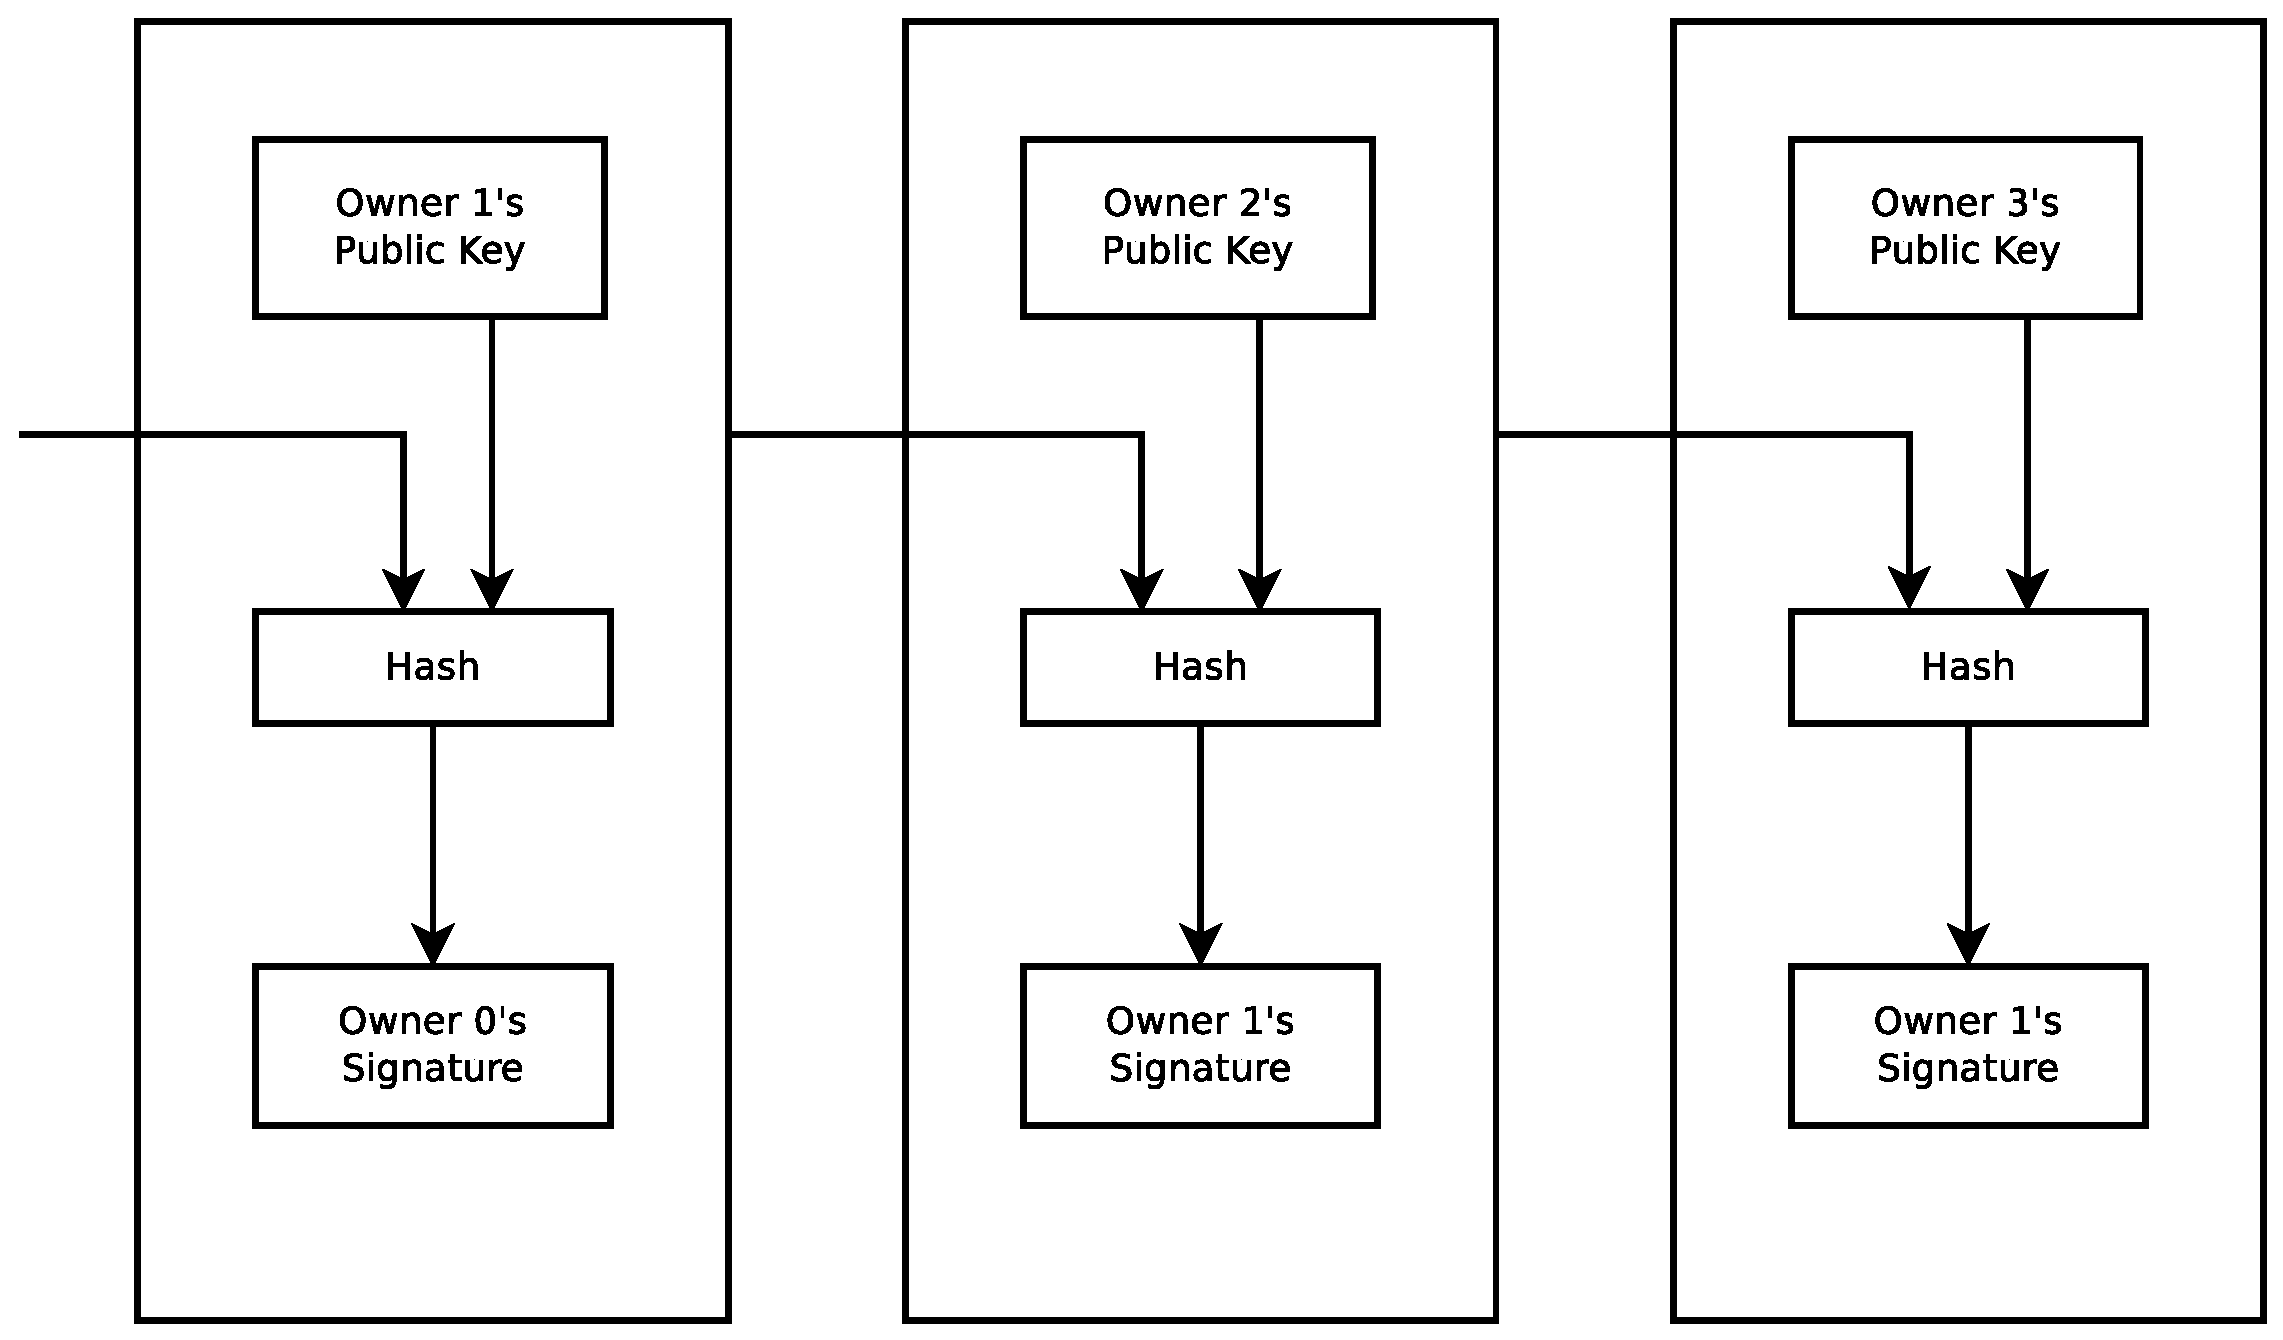
\includegraphics[scale=0.3]{problemDescription/figs/transactions.eps}}
	\caption{Transaction chain}
\end{figure}

Multiple transactions are aggregrated into a single block.
The next block is chained to the previous block by adding the hash of the previous block.
These blocks are created by nodes in the network, so called miners.
A miner receives transactions from other nodes in the Bitcoin network.
But the transactions are received in a non deterministic way induced by network characteristics.
The non deterministic nature causes blocks to differ from miner to miner.
The order of transactions has to be agreed upon by the network to eliminate this inconsistentcy.

Bitcoin uses election based upon Proof-Of-Work system.
To every block a nonce is added. 
This nonce is just a number that can be varied,
but is only sound if the result of the hash of the whole block starts with a certain number of zeros.
The amount of zeros required will be discussed later.
